\documentclass[a4paper]{article}

\usepackage[english]{babel}
\usepackage[utf8]{inputenc}
\usepackage{amsmath}
\usepackage{graphicx} 
\usepackage{caption}
\usepackage{subcaption}
\usepackage[colorinlistoftodos]{todonotes}
\usepackage[sort, numbers]{natbib} %Use bibtex package
\usepackage{url}
\usepackage{}
\usepackage{float}
\bibliographystyle{unsrtnat}
\renewcommand{\bibsection}{} %Remove default bibliography title
\newcommand{\HRule}{\rule{\linewidth}{0.5mm}}

\title{\huge GPS Journeys}

\begin{document}

% Title
%\HRule \\[0.4cm]
%{ \huge \bfseries GPS Journeys \\[0.4cm] }

%\HRule \\[1.5cm]

%\textsc{\Huge GPS Journeys}\\[1.5cm]




\author{Jack Crago, Ben Goss, \\ Megan Harrison and Sarah Pulfrey-Taylor}

\date{\today}

%\begin{document}

\maketitle


\begin{abstract}

This project presents methods of analysing GPS data used in finding unusual behaviours in tracking data of employees from a company called GAStech.. 
%what is done in the report
Methods to improve imperfect data are used, as the supplied data has missing entries. This report also produces results from clustering the data to find unusual behaviours by the employees. The GPS data is  split in to journeys, and each journey is analysed to identify which show normal behaviours and which are unusual. The journeys are  analysed to find the probabilites of an employee travelling from one location to another, which is used to predict their next movement.  



\end{abstract}

\pagenumbering{gobble}
\clearpage

\tableofcontents
\pagenumbering{gobble}
\clearpage

\pagenumbering{arabic}

\section{Introduction}
\label{sec:intro}

%What data is supplied

%main areas of investigation
%What methods are used
% AIMS AND OBJECTIVES OF THE PROJECT
% Aims are what you want to achieve, while, objectives are what you will do to achieve them. An objective is more specific in character, while an aim is more abstract. Also, an objective is time-bound whereas an aim need not be.


% The use of GPS systems has grown exponentially over the last 15 years, both on a personal and commercial level. Therefore large stores of GPS data are readily available, from anything between a smart phone and a tracking device, and highly useful information can be extracted. The aims of this project are to define the typical behavioural patterns of GAStech employees and hence extract behaviours that do not follow the trend.\\
% \noindent The objectives are to use various data analysis techniques to find this anomalous behaviour, and to draw conclusions from these results to identify whether or not these anomalies are substantial. 

%objectives - 
%Aims - To find outliers in the data, 
Large stores of GPS data are now readily available, with the development of smart phones and tracking devices. From apps that suggest running routes to car insurance prices dependent of the quality of the driver stem from GPS data analysis, and it is an increasingly important field of research.  For this project data is given by GAStech in order to investigate the disappearance of several employees shortly after the public offering of shares of the company. The data available is only for the two weeks prior to the disappearance excluding the day in question.

\subsection{Aims and Objectives}

The aim of this project is to identify typical behaviour of GAStech employees and hence identify unsual patterns within the data, so suspects linked with disappearance can be identified. To do this, imperfections such as missing data, have to be rectified. Data regarding the spending from different accounts must also be utilized to find patterns. The difference between unusual patterns in the data and anomalies that bear no significance to the invistigation must also be established. 

\section{Interpreting the Data}
\label{sec:datainterpret}


GAStech has given a large quantity of data  in order to identify unusual patterns of behaviour that may be related to the missing staff. This consists of various information about the different employees, including GPS tracking data, their credit card usage and loyalty card usage.

\subsection{Data Provided}
\label{sec:dataprovided}

The Car ID Assignment and Job Role data consists of the first and last names of the employees whose vehicles are tracked, and also their department, their employment title and an ID number associated with their vehicle. \\

\noindent However there are nine employees, all of whom are truck drivers, who do not have a car ID assigned to them. As a result it is not clear which route belongs to which truck driver, meaning that there is some uncertainty within the data. This problem is approached in section~\ref{sec:completedata}. \\

\noindent GPS tracking data is also supplied for 40 different company vehicles.  This data consists of latitude, longitude, a timestamp, and a vehicle ID number to link these vehicles back to people. It is the largest dataset supplied; it holds 14 days worth of GPS Tracking data for each ID. It allows the exact location of each vehicle supplied by the company to be known whenever the vehicle is moving, and also at what time this vehicle is moving. \\

\noindent The credit card data includes a timestamp to show the time of the transaction and establishment names to show where the transaction takes place. It also states how much was spent and who is using the credit card. Unlike the GPS data, this set gives a name as opposed to an ID number, which means that in order to link this data with the GPS data, the car ID assignment data must be cross-referenced and transactions must be matched to each employee. \\

 It is necessary to complete the data to allow a thorough analysis of the employees’ behaviours as the data provided is incomplete,. The locations of the establishments where credit cards and loyalty cards are used are unknown, as is the exact Identification of the truck drivers. Additionally the credit card data, loyalty card data and tracking data is of different resolutions. The tracking data gives the time to the nearest second, the credit card data gives the time of the transaction to the nearest minute, while the loyalty card data only gives the day of the transaction. The loyalty card data gives no assistance when finding the exact location of the establishments due to the low resolution. \\

\subsection{Initial Analysis of the Data}
\label{sec:initialanalysis}

Figure~\ref{fig:gpsdata} shows all of the GPS data for all employees with a company vehicle. There are some denser areas, near the centre of the graph, from this it can be deduced that people tend to make the same kind of journeys each day. There are also some journeys which are singular, and these are shown on the graph by the areas with sparse data. These are the journeys that need to be sought out as they are more likely to be the anomalies. \\

\begin{figure}[!ht]
\centering
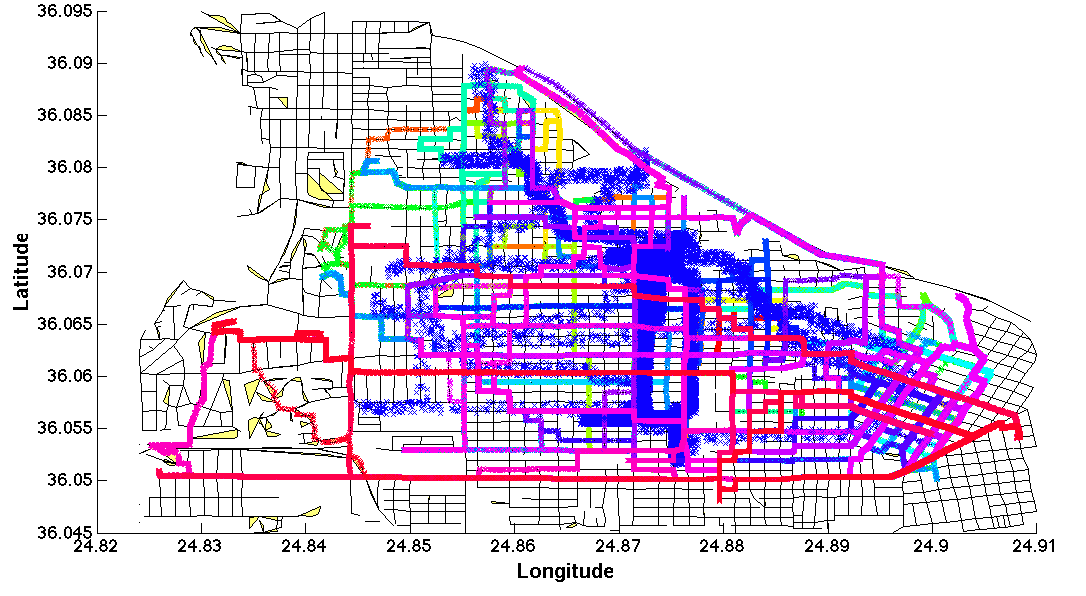
\includegraphics[width=0.9\textwidth]{gpsdata.png}
\caption{\label{fig:gpsdata}A plot showing all GPS data provided.}
\end{figure}


\noindent  Figure~\ref{fig:spending} shows the spending patterns of the employees. The cluster of lines towards the bottom of the graph shows that most employees have a similar spending pattern. There are ten employees who spend much more. The majority of these outliers are truck drivers, who spend a lot of money on fuel, however there is one outlier, Lucas Alcazar who is an IT Helpdesk assistant who spent a total of 11,454.00 which is unusually high in comparison to other employees with the same job. \\
\begin{figure}[!ht]
\centering
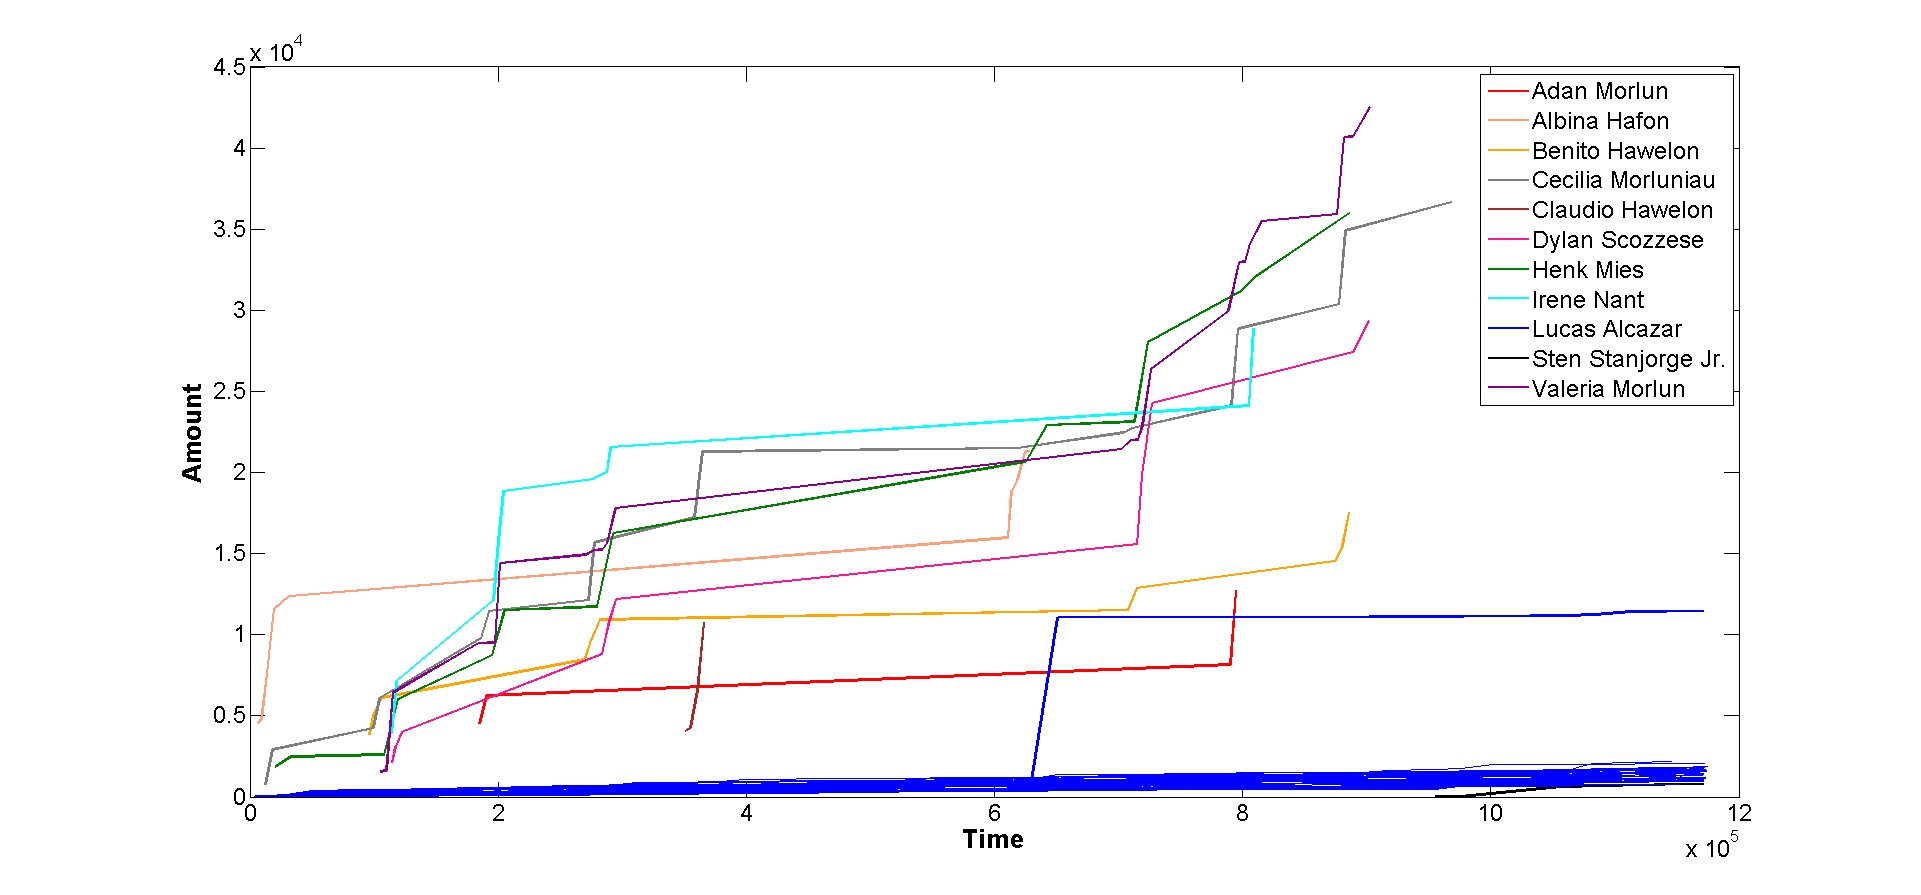
\includegraphics[width=1.0\textwidth]{spending.png}
\caption{\label{fig:spending}Total amount spent on each person's credit card.}
\end{figure}





\section{Completing the Data}
\label{sec:completedata}
\subsection{Coordinates of Establishments}
\label{sec:completeloc}

\noindent To find the locations of the establishments the credit card data of all employees with a company vehicle is studied in closer detail. As the tracking software only gives data while the vehicle is moving there is often no data given for the minute in which the transaction takes place. This can be explained by people parking their vehicle, then using their card, before returning and driving away.  To find the coordinates of the establishment the closest time either side of the transaction is recorded and the corresponding coordinates recorded and averaged to give the coordinates of the establishment. This is repeated for all transactions made by employees with company vehicles allowing a set of coordinates to be found for each identified location. This allows outliers to be removed and give more accurate coordinates for the establishment. This error could be produced by a number of factors. As already mentioned the different resolutions may produce error, another source of error could be produced by people parking their vehicle away from the establishment and walking. 
 
 \subsection{Identifying Truck Drivers}
 
This method only allows the coordinates of some establishments to be found. This is because certain establishments are only visited by employees without a company vehicle or by employees driving a company truck. To overcome this problem the trucks need to be linked to an employee. The data gives the names of all employees that use a truck but does not say which truck they use.
The credit card transactions, by employees in a truck, at known establishments are used to find which truck is at that establishment.
The complete truck allocation is shown in Table \ref{table:truck_drivers}. This additional information allows the coordinates for the remaining establishments to be found.

\begin{table}[H]
\begin{center}
\begin{tabular}{|l|l|l|}
\hline
Vehicle ID & First Name & Last Name \\ \hline \hline

36 &Albina & Hafon\\ \hline
36&Benito& Hawelon\\ \hline
36&Claudio& Hawelon\\ \hline
37&Henk&Mies \\ \hline
38&Valeria&Morlun \\ \hline
39&Irene& Nant\\ \hline
39&Dylan& Scozzese\\ \hline
40&Adan& Morlun\\ \hline
40&Cecilia& Morluniau\\ \hline


\end{tabular}
\caption{\label{table:truck_drivers}Vehicle ID numbers matched to employees.}
\end{center}
\end{table}


	
	
	
	


\section{Clustering Method for Outlier Detection}
\label{sec:clusteroutlier}

It is important to detect outliers, to identify unusual behaviours shown by the employees. These outliers can also be used to highlight any possible imperfections in the data.

\subsection{Distance Measurement}
\label{sec:euclidean}

The definition of distance measurement between two data points is highly important in such a project, which uses spatial data. This project uses Euclidean distance and the distance $d(\bf{p},\bf{q})$ and is given in equation \ref{euclid}

\begin{equation}
\label{euclid}
d(\bf{p},\bf{q}) = \sqrt{(\bf{p}-\bf{q})\cdot(\bf{p}-\bf{q})}
\end{equation}



\subsection{Time of Day Comparison}
\label{sec:outliertimeday}

Data of interest is the comparison of the total distance travelled at different times of the day during the 14 day period. For this type of analysis the total distance travelled on weekends has been removed from the data set, since weekday travelling patterns often differ distinctly from weekend travelling patterns. The two times of day that are compared are 10.00 am and 4.00 pm. The first time has been selected in order to contain all distance travelled from home to work. The second is chosen to include all travel within lunch hour activities, but to exclude all travel to home. The total distance travelled in the morning in comparison to the afternoon for each vehicle on each day over the two week period is collated and shown in Figure \ref{fig:mornaft}. 

\begin{figure}[!ht]
\centering
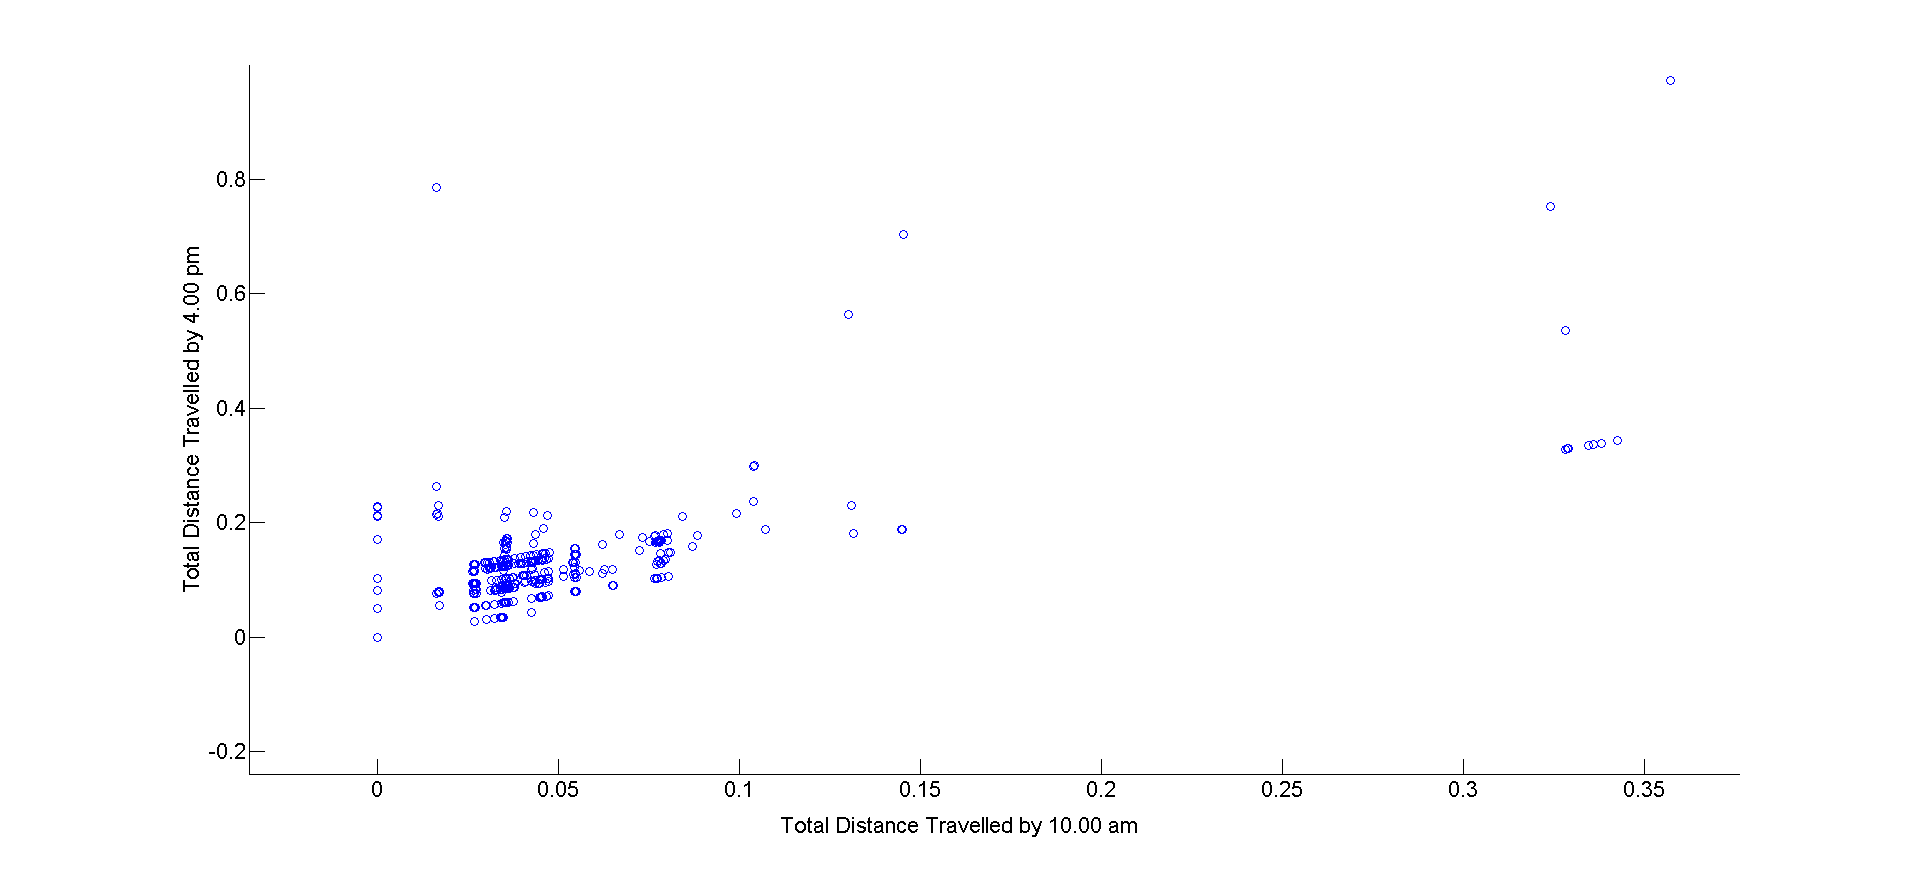
\includegraphics[width=1.1\textwidth]{Images/1stoutlier.png}
\caption{\label{fig:mornaft}Scattergraph showing total distance travelled at 10.00 am versus 4.00 pm for all vehicles for each weekday.}
\end{figure}

\noindent In Figure \ref{fig:mornaft} a high density area of data points can be seen with multiple outliers. To detect these outliers a method of cluster analysis can be used, and k-means clustering has been chosen for this set of data.



\subsection{K-means Clustering}
\label{sec:kmeans}

\noindent  K-means clustering is a centroid based classification system, and works by  creating number $k$ centroids, which are random points within the space.   Each of the $n$ observations into one of $k$ clusters; the cluster with the nearest mean in distance. The mean is then recalculated from these new clusters, and the algorithm repeats until the centroids no longer move location. A local optimum has been found. K-means clustering again relies on Euclidean distance. However a drawback of the k-means clustering set is the number of clusters within the data set must be determined beforehand. 



\subsection{Determining Number of Clusters}
\label{determinenocluster}


One approach to determine the appropriate number of clusters is to look at the within class variance $\sigma^2_{W}$ and between class variance $\sigma^2_{B}$, which are given in equations (\ref{OB}) and (\ref{OW}) . $N$ is the total number of data points, $K$ is the number of clusters and $C_{k}$  is the number of elements in cluster k. Lastly $\bar(x)$ is the mean of all data.
\begin{equation}
\label{OW}
\sigma^2_{W} = \frac{1}{N}\sum_{k = 1}^{K}\sum_{i = 1}^{C_{k}}[(x_{i} - \mu_{k})(x_{i} - \mu_{k})^T]
\end{equation}

\begin{equation}
\label{OB}
\sigma^2_{B} = \frac{1}{N}\sum_{k = 1}^{K} C_{k}[(\mu_{k}-\bar{x})(\mu_{k}-\bar{x})^T]
\end{equation}


\noindent It is desirable that a clustering algorithm produces results where each cluster is of a high density, and each cluster is far removed from any other cluster. In other words, the optimisation problem is to minimise $\sigma^2_{W}$ and to maximise $\sigma^2_W$. However the sum of within- and between- class variance is equal to the variance of the data, which is constant. Hence minimising $\sigma^2_{W}$ and maximizing $\sigma^2_W$ is the same optimisation problem, and the focus can be placed on $\sigma^2_{W}$ . The plot of the number of clusters versus $\sigma^2_{W}$ is shown in Figure \ref{fig:elbow}.\cite{cluster}



%will change this graph in the morning
\begin{figure}[!ht]
\centering
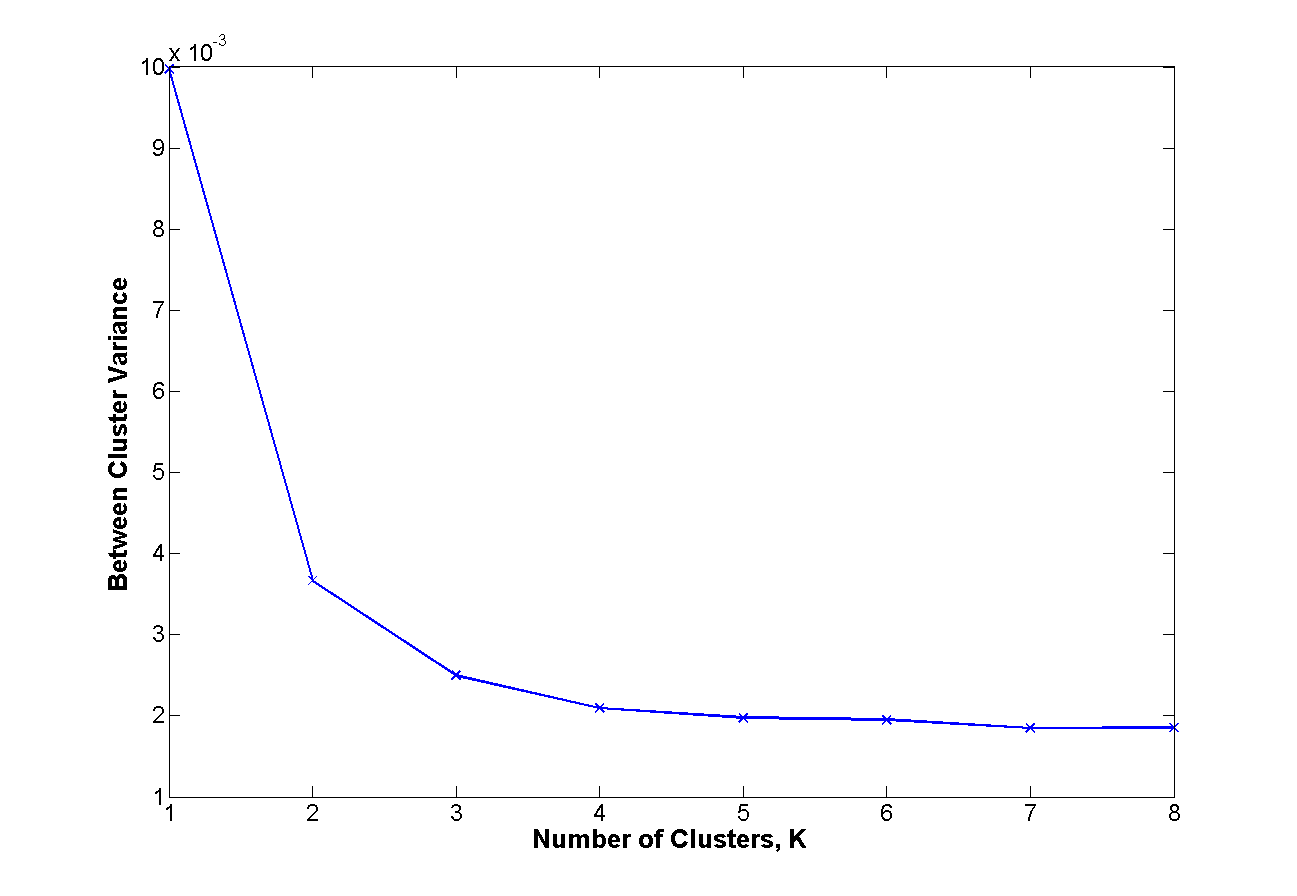
\includegraphics[width=1.0\textwidth]{Images/Sw2graph.png}
\caption{\label{fig:elbow} Graph showing the relationship between number of clusters and Between-class Variance  }
\end{figure}






% %will change this graph in the morning
% \begin{figure}[!ht]
% \centering
% 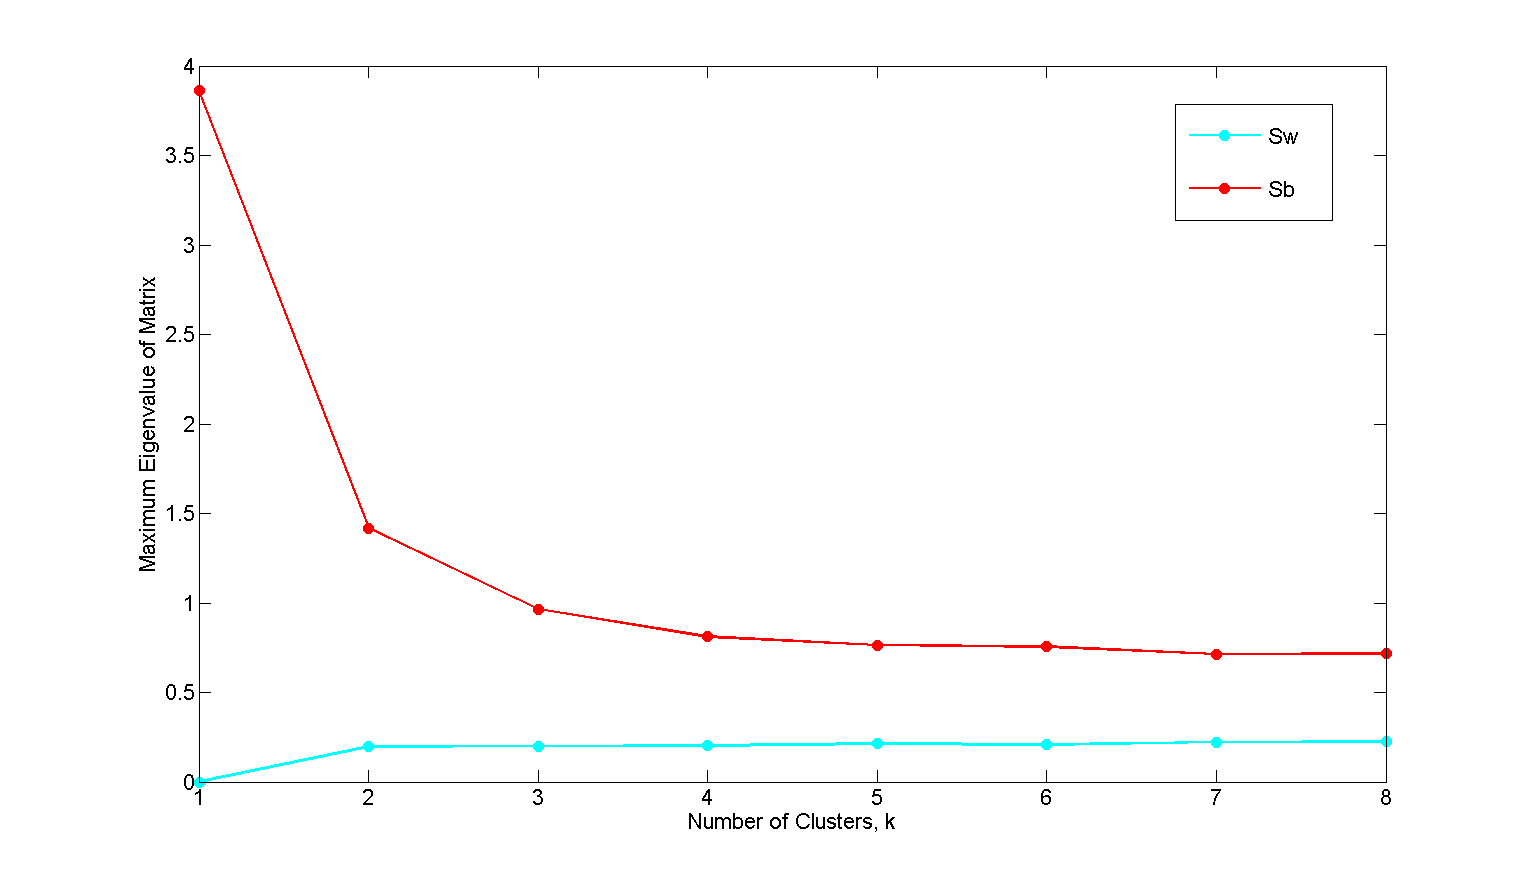
\includegraphics[width=0.8\textwidth]{Images/Swsbgraph.png}
% \caption{\label{fig:elbow} Number of Clusters against the maximum eigenvalue of the scatter matrix }
% \end{figure}



\noindent Figure \ref{fig:elbow} shows that $\sigma^2_{W}$ decreases as the number of clusters increases. This will continue until $K = N$, where each data point is defined as a cluster.\\

\noindent However, a trade off between model accuracy and complexity should be taken into account and so the elbow point should be studied. The elbow point for $\sigma^2_{W}$ is $K = 3$ and so this should be taken as the appropriate value for the model. The clustering algortithm with $k  =3$ is shown in Figure \ref{fig:4cluster}.



\begin{figure}[!ht]
\centering
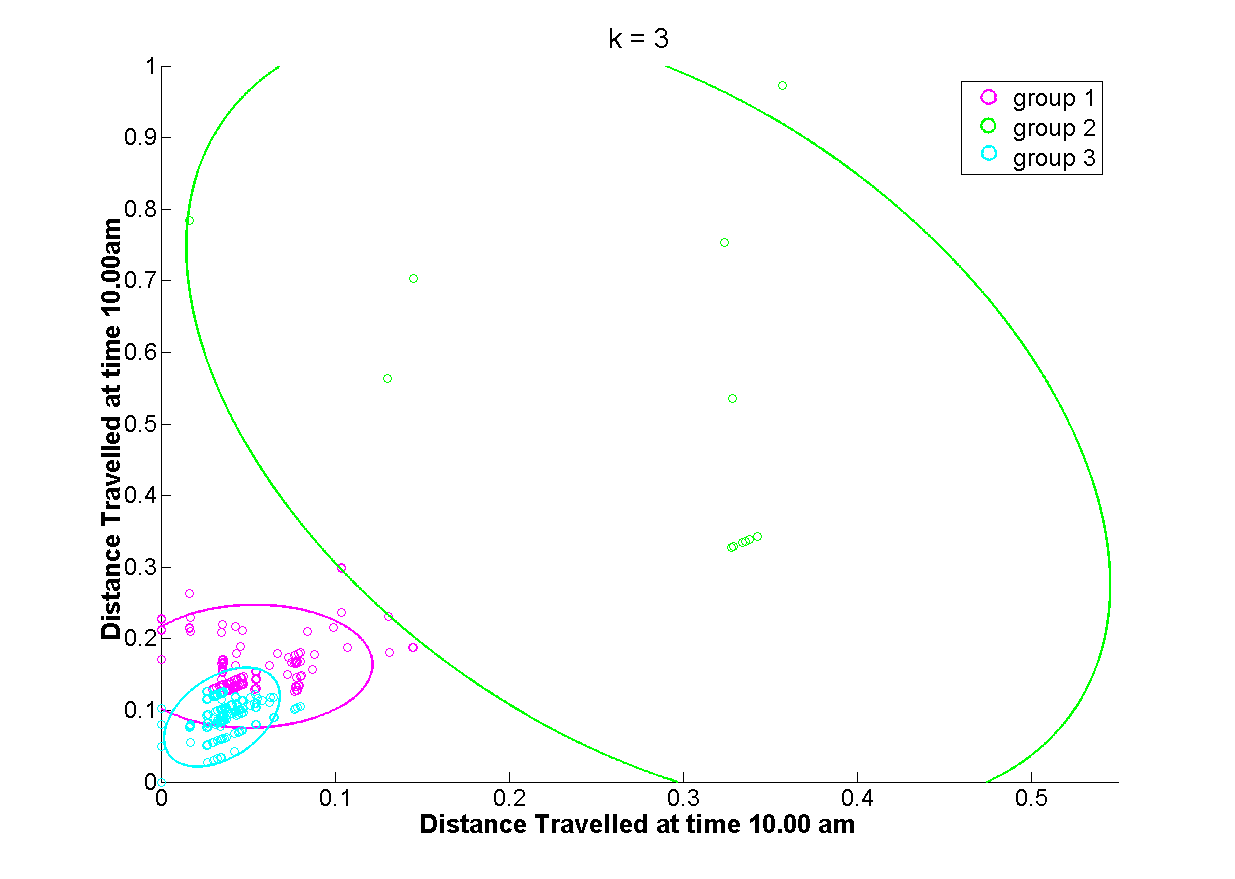
\includegraphics[width=0.7\textwidth]{Images/4cluster.png}
\caption{\label{fig:4cluster} Results of k-means clustering with k = 3. Ellipses contain 95\% of the data within the cluster.}
\end{figure}





\subsection{Outlier Identification}
\label{sec:outliers}
From the results of the k-means clustering the outliers can be identified. It can be seen that members in group 2 are outliers. This is because the two other groups have a visibally smaller within cluster variance , and group 2 is much bigger and removed. These values are summarised in Table \ref{table:outliers}. Further investigation will be carried out on Elsa Orilla, as she is consistently travelling a much further distance than any other individual, which can been seen in section 5.2.


\begin{table}[H]
\begin{center}
\begin{tabular}{|l|l|}
\hline  
Person & Day  \\ \hline \hline
Elsa Orilla     &   1,2,3,4,5,8,9,10,11,12   \\ \hline
Willem Vasco-Pais    &  5,11   \\ \hline
Valeria Morlun, Adan Morlun, Cecili Morluniau&    12   \\ \hline

\end {tabular}
\caption{\label{table:outliers}Outliers identified by K-means Clustering Method}
\end{center}
\end{table}

%\clearpage





\section{Journey Analysis}
\label{sec:journeyanalysis}
\subsection{Time of Movement}
\label{sec:timeofmovement}

To find patterns in the time of employees’ movements a graph showing when an employee moved is plotted. The time in Figure \ref{fig:MoveTime} begins at the time of the first GPS data point. If an employee moves during an hour a point is plotted. The colour of the marker indicates the employees current employment type. Yellow indicates an information technology worker, blue indicates an engineer, red indicates an executive, cyan indicates a security worker and green indicates a truck driver.   

\begin{figure}[H]
\centering
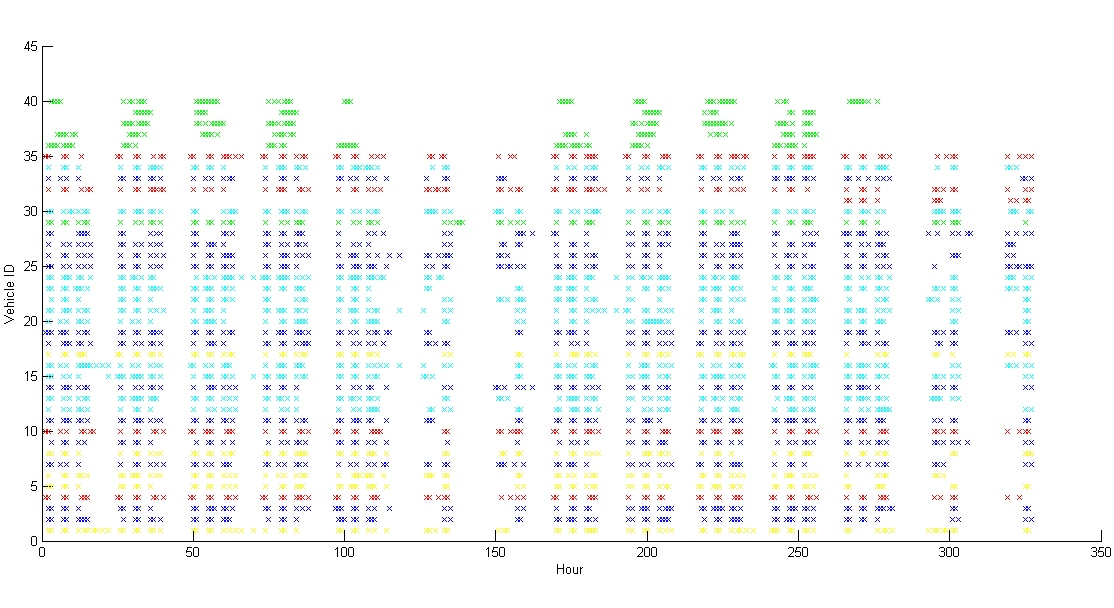
\includegraphics[width=1.2\textwidth]{MoveTime.jpg}
\caption{\label{fig:MoveTime}A data point shows a vehicle ID moved in that hour.}
\end{figure}


\noindent Figure \ref{fig:MoveTime} shows a number of interesting patterns. Most employees move during the day and then have a period overnight when they don’t move, as expected. However, it can be seen that some employees move in the day, then continue to move when most other employees stop. There are five employees showing this unusual pattern in their movements, they are identified in table \ref{table:time_ids}. \\


\begin{table}[H]
\begin{center}
\begin{tabular}{|l|l|l|}
\hline
Vehicle ID & First Name & Last Name \\ \hline \hline

1 &Lucas & Alcazar\\ \hline
15&Loreto&Bodrogi\\ \hline
16&Isia& Vann\\ \hline
21&Hennie&Osvaldo \\ \hline
24&Minke& Mies

\end{tabular}
\caption{\label{table:time_ids}Employees showing unusual patterns in their movement.}
\end{center}
\end{table}

\noindent To investigate this behaviour the tracking data for each employee is split into individual journeys to give an insight into where these employees are travelling. A journey enda if a vehicle does not move for more than 10 minutes. When these journeys are plotted, as shown in Figure \ref{fig:TimeJourneys},  it can be seen that vehicles 15, 16, 21 and 24 all start in a similar area and make very similar journeys. Vehicle 1 appears to make a set of journeys that are independent of the other 4 vehicles, so these patterns are considered as 2 different anomalies. 

\begin{figure}[H]
\centering
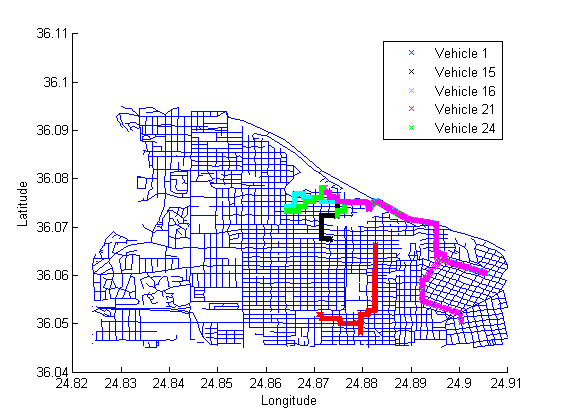
\includegraphics[width=0.9\textwidth]{TimeJourneys.png}
\caption{\label{fig:TimeJourneys}The journeys made at unusual times.}
\end{figure}

\subsection{Clustering Journeys}
\label{sec:clusteringjourneys}

\noindent To see locations frequently visited, clustering is applied to the start and end points of the journeys. Agglomerative hierarchical clustering is used, this is preferred to k-means clustering as the number of clusters in the data is unknown. Figure \ref{fig:Clustering} shows the clusters found that contain 5 or more data points. The threshold is set at 5 data points as this removes the small clusters and leaves the most frequently visited clusters. Most locations with credit card transactions have a large cluster around them, and there is also a large cluster around what is believed to be the Gastech office. There are also clusters that appear to be the homes of the employees, they are usually visited by one employee and are the last place visited at the end of the day. \\

\begin{figure}[H]
\centering
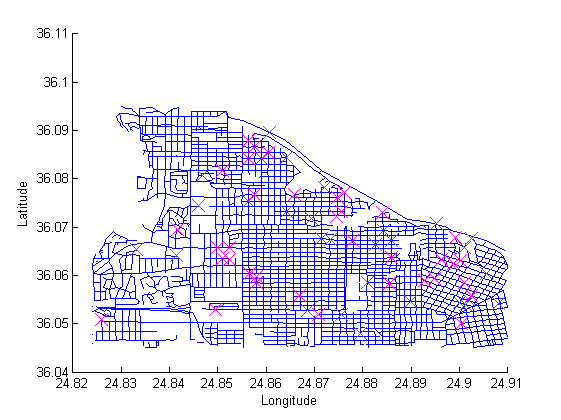
\includegraphics[width=1.1\textwidth]{Clustering.png}
\caption{\label{fig:Clustering}Clusters with 5 or more data points found using agglomerative hierarchical clustering.}
\end{figure}

\noindent When comparing these clusters to the unusual journeys it is seen that all of these unusual journeys start and end at a cluster. The first night of unusual activity by vehicle 1 shows the employee travelling from their home to the office and then back to their home. On the second night of unusual behaviour the employee travels from an establishment identified as Ouzeri Elian, to the office and then to their home. This doesn’t match the behaviour of any other employee and is consider as an anomaly.\\

\noindent Vehicles 15, 16 and 21 all start their unusual journeys from the same cluster, there are no establishments at this location and it is not known what is there. This cluster is also visited by one other employee in vehicle 13. Vehicle 24 starts from a different cluster, again there are no establishments at this location, this cluster is also visited by vehicles 17 and 33. The vehicles then travel to 4 different clusters, each of these clusters is visited by 3 different people, 2 from the set of employees being investigated and one executive. On further investigation it appears these clusters are the executives’ homes as they are regularly visited by the executive and are the last place visited at the end of the day. Table \ref{table:watch_table} shows a summary of these visits.


\begin{table}[H]
\begin{center}
\begin{tabular}{|l|l|l|}
\hline
Executive & First Employee & Second Employee \\ \hline \hline

Ingrid Barranco &Loreto Bodrogi &Isia Vann \\ \hline
Ada Campo-Corrente&Loreto Bodrogi&Minke Mies\\ \hline
Orhan Strum&Isia Vann& Hennie Osvaldo\\ \hline
Willem Vasco-Pais&Hennie Osvaldo& Minke Mies\\ \hline
\hline

\end{tabular}
\caption{\label{table:watch_table}A summary of employees at exectives' houses.}
\end{center}
\end{table}


\noindent To find any further connection between the four employees being investigated and the three employees that appeared at the start points of the unusual journeys all clusters visited by three or more of the employees being investigated are found. Five clusters are found that contain only a subset of the employees being investigated as well as Inga Ferro in vehicle 13, as shown in Figure \ref{fig:Watch_Clusters}. This suggests that there is a connection between Inga Ferro and the other employees being investigated. There appears to be no further connection between vehicles 17, 33 and the employees being investigated as there are no additional clusters containing a subset of the employees being investigated and these vehicles. 

\begin{figure}[H]
\centering
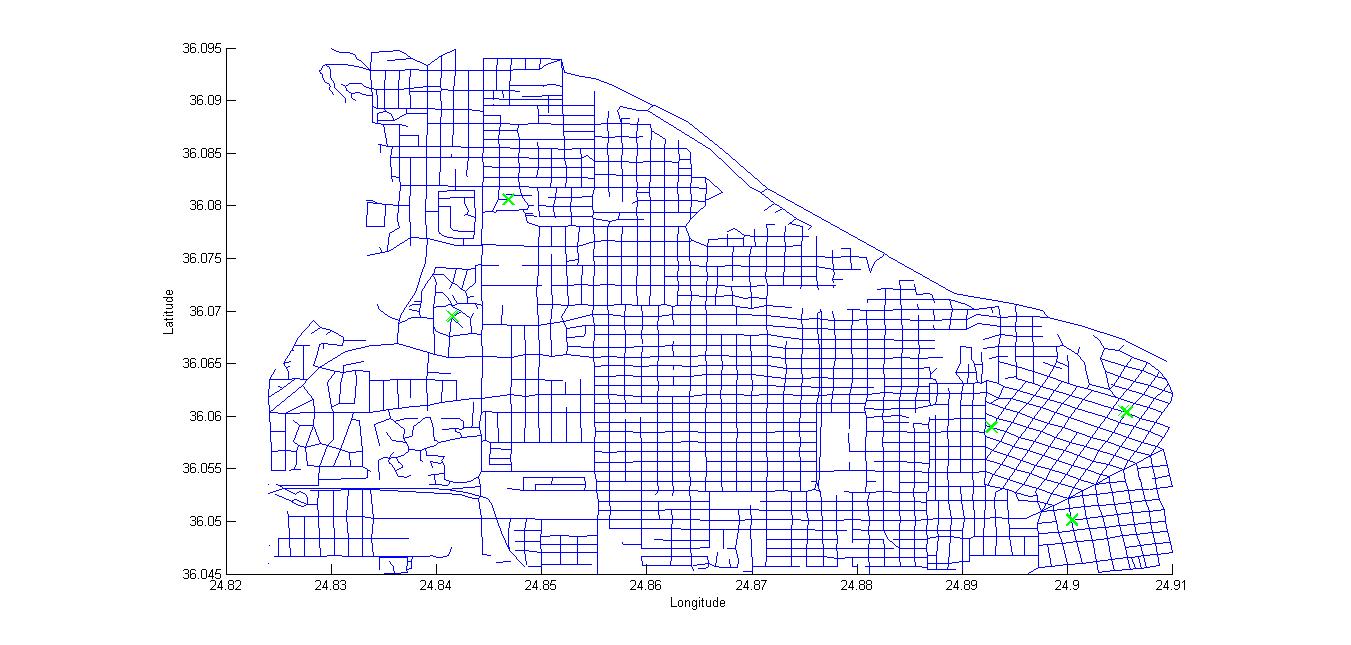
\includegraphics[width=0.9\textwidth]{Watch_Clusters.png}
\caption{\label{fig:Watch_Clusters}Clusters only visited by a subset of the suspect individuals.}
\end{figure}

\noindent To continue on the results in section 4 clusters visited by Elsa Orilla are investigated. It is discovered that Elsa Orilla in vehicle 28 uniquely visits 4 clusters.  These clusters are shown in Figure\ref{fig:ID28_Clusters}, there are no known establishments at these locations. 

\begin{figure}[H]
\centering
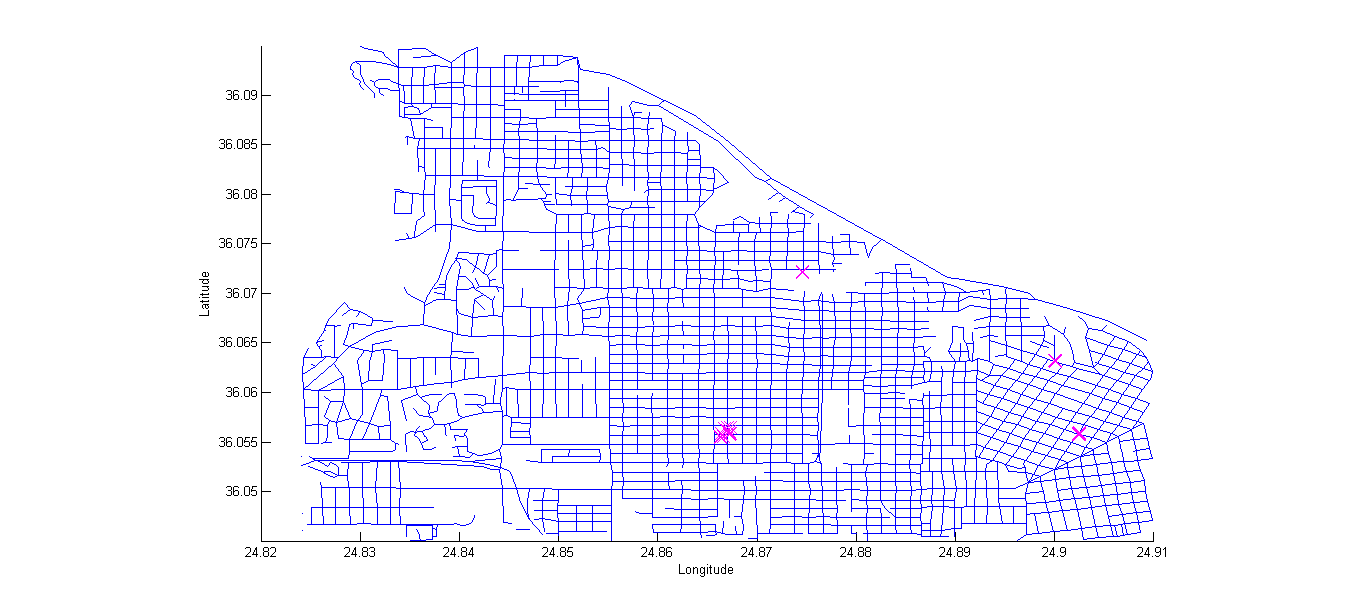
\includegraphics[width=0.9\textwidth]{ID28_Clusters.png}
\caption{\label{fig:ID28_Clusters}Clusters only visited by Elsa Orilla.}
\end{figure}




\section{Correlations}
\label{sec:correlations}

\noindent The correlation coefficient is a measure of the linear dependence between two variables and is calculated as follows:

\begin{equation}
r = \frac{\sum_{i=1}^{n}(X_i - \bar{X})(Y_i - \bar{Y})}{\sqrt{\sum_{i=1}^{n}(X_i - \bar{X})^2}\sqrt{\sum_{i=1}^{n}(Y_i - \bar{Y})^2}}
\end{equation}

\noindent where $r$ is the correlation coefficient and has a value between +1 and -1.

\noindent If $r$ = +1 it corresponds to a positive perfect correlation as $X$ increases so does $Y$. Similary if $r$ = -1 it corresponds to a negative perfect correlation, as $X$ increases $Y$ decreases. A correlation coefficient of 0 means that there is no correlation between the two variables. \cite{corrcoeff}.


\subsection{Distances Travelled}
\label{sec:corelldistance}

Using an outlier that has previously been found, in this case Elsa Orilla, the distance data from such outlier can be compared for each day in order to have another form of analysis to confirm that it is an anomaly. \\

\begin{figure}[H]
\centering
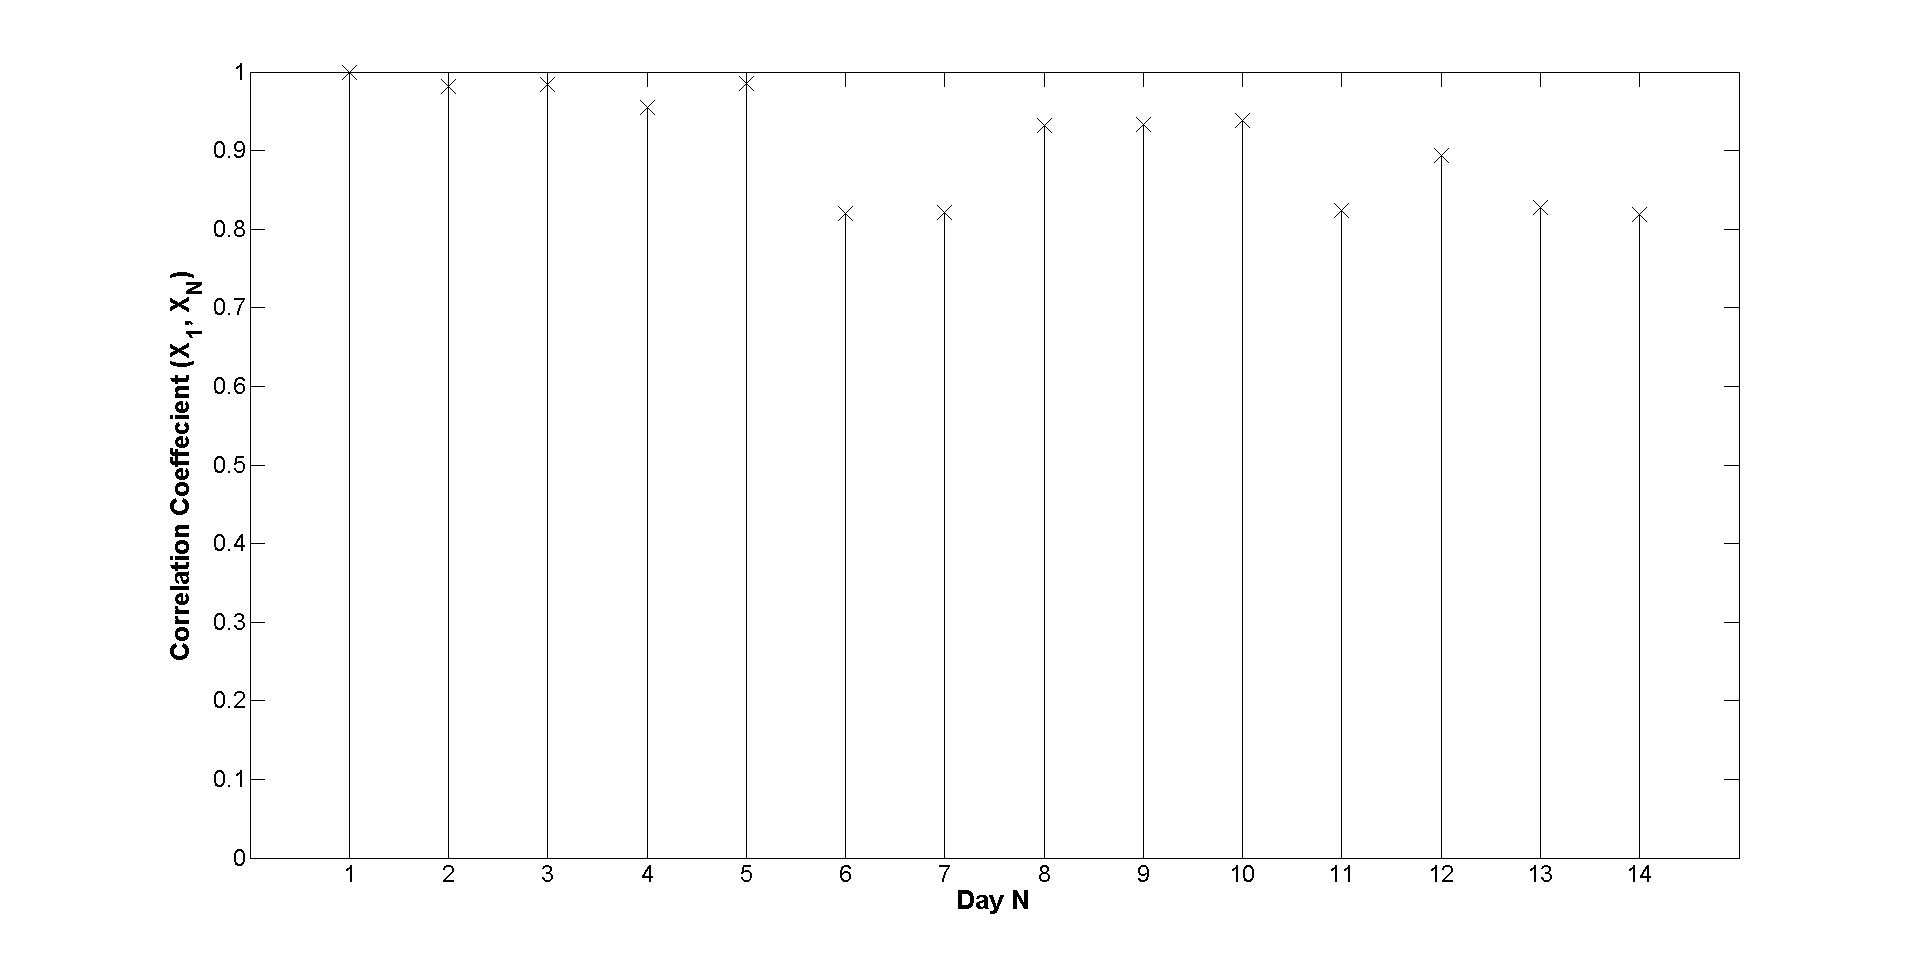
\includegraphics[width=1.0\textwidth]{CorrelateDistanceID28.png}
\caption{\label{fig:CorrelateDistanceID28} The correlation coefficients, for distance travelled by Elsa Orilla, between day 1 and day 14.}
\end{figure}

\noindent Figure \ref{fig:CorrelateDistanceID28} shows this correlation. The distance data is correlated in such a way that each day is compared to the first day in the time period. From Figure \ref{fig:CorrelateDistanceID28}  it can be seen that each day has a fairly high correlation coefficient, however this is to be expected because the distance will always be increasing as it is the cumulitive distance. Nonetheless there are some values that are significantly lower than others and this shows that on the day where such a value appears, the distances travelled were different to those travelled on day 1. \\ 


\section{Predicting Employee Behaviour}
\label{sec:predicting}

Predicting employees behaviour is a useful form of analyse for the supplied data.  

\subsection{Simple Model}
\label{sec:simplemodel}
\subsubsection{Defining Locations}
The first step in creating a probabilistic model is to choose the locations that will be used to calculate the probabilities from. \\
\begin{figure}[H]
\centering
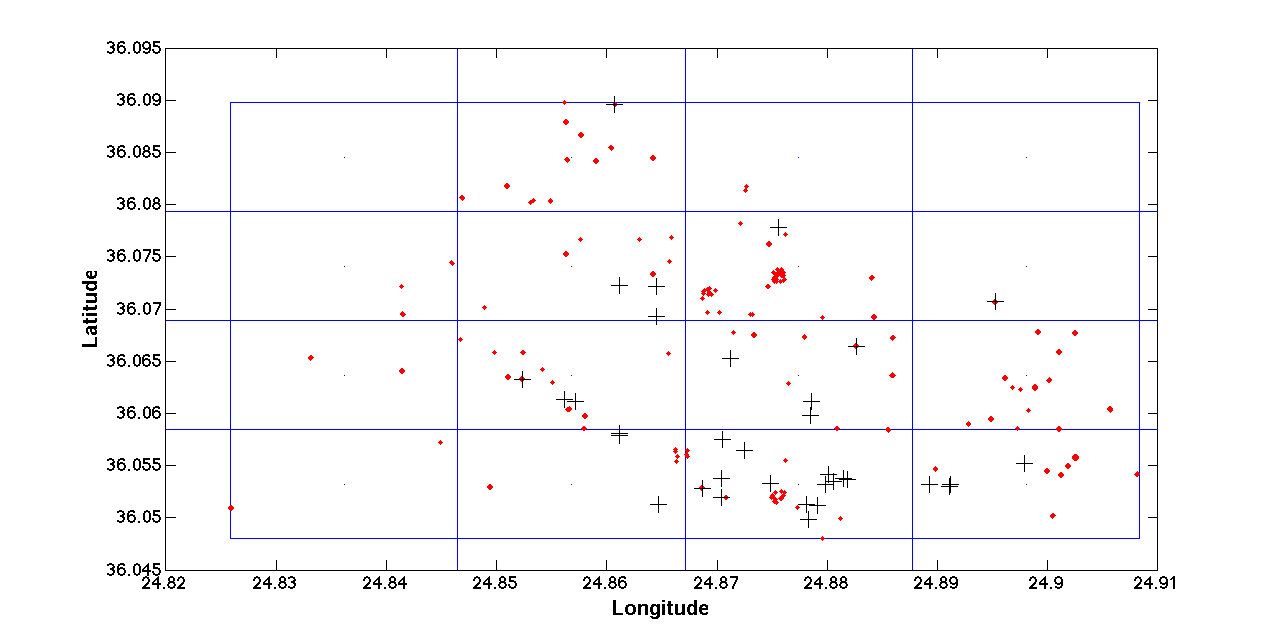
\includegraphics[width=1\textwidth]{locationbound.png}
\caption{\label{fig:locationbound}A graph showing the boundaries created for 16 areas, and the start and end points of all journeys. }

\end{figure}
\noindent This method involves splitting Abila up in to sectors, which is done using the minimum and maximum points from the data, and using these as the boundaries. A set of equidistant points are then selected along the x and y axis, which are used as the corners of the boundaries. From this rectanglar boundaries are created to distinguish between the different regions, as shown in Figure \ref{fig:locationbound}. Each region is labelled and all points that fall within this region are assigned this class. The regions are labelled from 1 to 16 with the lower left corner labelled as 1 and the upper right corner labelled as 16. 

\noindent An important factor with this type of model is to consider how many clusters to use. For the simple model, using 16 clusters in a 4x4 grid is chosen, as there are 34 known locations in the GPS data (see Section \ref{sec:completeloc} ), and if each known location shares a cluster with one other known location, that leaves 17 clusters, to which 16 is the nearest square number.
%Finish this section - I picked 16. Why? What made me do that?

\subsubsection{Calculating Probabilities}

When creating an ideal probabilistic model, the probability of travelling to another location will be dependent on various factors, such as the time of day. A simplified model is assumed, where the probability of an employee travelling to another region is dependent on regions the employee has been before. This is shown in Equation \ref{eq:probtot} :
\begin{equation}\label{eq:probtot}P(l_n | l_{n-1}, l_{n-2}, l_{n-3}, ...),\end{equation}
where $l_n$ is the region of the employee at time $n$. In this model the previous locations of the employee until $n=-\infty$ are taken into account for the probability calculation. As this is impossible to create, an assumption must be made, known as the Markov assumption shown in Equation \ref{eq:markovassumpt}\cite{markov}. %http://di.ubi.pt/~jpaulo/competence/tutorials/hmm-tutorial-1.pdf reference this here
\begin{equation}\label{eq:markovassumpt}P(l_n | l_{n-1}, l_{n-2}, ...)\approx P(l_n | l_{n-1})\end{equation}

\noindent This assumption is a First Order Markov Assumption, which means that only the previous location is considered when calculating the probability.\\
\noindent Using this assumption, the probabilities are calculated by summing the number of journeys from the start region to another end region. This is then divided by the number of journeys from the start point to any point  \cite{gpspredict}.\\ 
%reference gps report here
 

\subsection{Simple Model Analysis}
\label{sec:simpleanalysis}
%You need to do this section, you can't keep putting it off
%Talk about predicting
Predictions using this model can be calculated very simply, as each journey between two points is set a probability. Therefore, if there are four locations; A, B, C and D, the probability of someone travelling from A to B and then from B to C would just be the product of the two probabilities. \\
%Which journey has the highest probability of happening from each cluster?

\subsubsection{Analysing all GPS Data}
\begin{table}[H]
\begin{center}
\begin{tabular}{|l|l|l|}
\hline
Start Position & Most Likely End Position & Probability \\ \hline \hline
1  &   3   & 0.5000 \\ \hline
2  &   11  & 0.6000 \\ \hline
3  &    8  & 0.2207 \\ \hline
4  &    3  & 0.4892 \\ \hline
5  &    5  & 0.5625 \\ \hline
6  &    3  & 0.6939 \\ \hline
7  &    3  & 0.6128 \\ \hline
8  &    4  & 0.6774 \\ \hline
9  &    6  & 0.4615 \\ \hline
10 &    3  & 0.3595 \\ \hline
11 &   10  & 0.2366 \\ \hline 
12 &    3  & 0.6667 \\ \hline
13 &    1  & 0.0000 \\ \hline
14 &   10  & 0.3180 \\ \hline
15 &   11  & 0.5000 \\ \hline
16 &    1  & 0.0000 \\ \hline

\end{tabular}


\caption{\label{table:simplemodel}Results of probability calculations}
\end{center}
\end{table}

As can be seen from Table \ref{table:simplemodel}, the most probable region that people will travel to is 3. This could be explained as region 3 is the region that Gastech is located in. It also has the highest number of establishments that people used their credit cards in.


\noindent  The probabilities for area 16 is equal to 0 because there are no journeys that occur in either of those areas. This could be explained by region 16 being taken up mostly by  the sea.\\
%From work


\noindent In order to see where people are likely to travel from work, region 3 is used as the start point. The probabilities for a journey to each region are shown in Table \ref{table:fromwork}. This table shows that the four areas with the highest probability of being the target location from 3 are 8, 3, 4 and 6. 4 and 8 are the regions that restaurants are located in, so these being the highest probabilities suggests the employees leave work and go straight to a restaurant, whether at lunch or straight after work.

\noindent As for people from region 3 having a high probability of staying within region 3 when they travel, it is likely down to the fact that region 3 is full of places that people use their credit cards.

\begin{table}[H]
\begin{center}
\begin{tabular}{|l|l|}
\hline
End Location & Probability \\ \hline \hline
	1  &  0.0337 \\ \hline
    2  &  0.0000 \\ \hline
    3  &  0.1463 \\ \hline
    4  &  0.1394 \\ \hline
    5  &  0.0012 \\ \hline
    6  &  0.1394 \\ \hline
    7  &  0.0755 \\ \hline
    8  &  0.2207 \\ \hline
    9  &  0.0070 \\ \hline
   10 &  0.0732 \\ \hline
   11  &  0.0767 \\ \hline
   12 &  0.0105 \\ \hline
   13 &  0.0000 \\ \hline
   14  &  0.0767 \\ \hline
   15 &  0.0000 \\ \hline
   16 &  0.0000\\ \hline

\end{tabular}
\caption{\label{table:fromwork}Results of probability calculations from area 3}
\end{center}
\end{table}


\section{Conclusion}
\label{sec:conclusion}


In this report a selection of data analysis techniques have been applied to a dataset to identify patterns and predict behaviour. From this unusual behaviour has been identified and investigated to find employees that may be connected with the disappearance.  
The data provided was used to find the coordinates of the establishments where employees used their credit cards. A complete car assignment was also found by finding the exact identification of the truck drivers. \\

An anomaly was discovered in the spending patterns of the employees. One employee was found to spend considerably more money than any other employee with a similar job.

\noindent Analysis of the times when employees moved showed five employees moving at night when all other employees made no journeys. One of these employees was returning to the Gastech office, no other employees appear to work at night so this was identified as an anomaly. Clustering showed the four other employees were staying outside executives’ houses overnight and meeting with a fifth employee and five unknown locations. 

An employee was identified as travelling a greater distance than other employees. This was confirmed as an anomaly when it was discovered that this employee also uniquely visited four clusters.

Using the probabilities from Section \ref{sec:predicting}, region 3, which is the area that GAStech is located in, is shown to be the area that people frequent most often. This is understandable, as the majority of employees would have to go to the complex every day for work. From the area with GAStech, the next most likely location that they will travel to is area 8, which is full of restaurants and cafes. This is most likely because the employees would go for lunch, or to dinner straight after work. \\


\section{Further Development}
\label{sec:furtherdevelop}
%Checked this. i'm happy with it. SPT

\subsection{Credit Card Outliers}
\noindent The outliers identified when matching the vehicle tracking data and credit card data could be investigated further. Although these outliers may be the result of inaccuracies in the data they may show other interesting patterns or unusual behaviours by the employees. 

\subsection{Journey analysis}
To find more patterns in the journey data the small clusters could be analysed to find individuals making unique journeys. The journeys for each individual could also be analysed to find any routines shown by individuals, this would allow any change in this routine to be identified as an anomaly.

\subsection{Prediction}
In order to predict the location change of an employee more accurately, the simple model can be made more elaborate. 

\subsubsection{Second Order Markov Model}
The first way of making the model more complex is to use a Second Order Markov Assumption, as shown in Equation \ref{eq:markovassumpt2} below. 

\begin{equation}\label{eq:markovassumpt2}P(l_n | l_{n-1}, l_{n-2}, ...)\approx P(l_n | l_{n-1}, l_{n-2})\end{equation}

\noindent This assumption makes the model more accurate, and also more complex, as the model takes previous behaviour into account more, but it also means that the amount of probabilities needed to be calculated increases to the power of 3. This causes more computing power to be needed, and also makes the results more complicated to analyse.


%%JACK, GOT BACK FROM ORCHESTRA AND WORKING ON IT> THOUGHT THIS BIT SHOULD BE JUST COMMENTED OUT, FEEL FREE TO CHANGE IT. SARAH.


% \subsubsection{Clustering Peoples Locations}
% Another modification that can be made to the simple model in order to make the results more realistic is for the clusters of people (known as areas above) to dynamically resize rather than for them to just be a static size. This can be done by various algorithms, including k-means clustering,  explained in Section \ref{sec:kmeans}. If using the k-means, the number of centroids has to be chosen. Then, the points can be clustered using the algorithm. Then, the probability calculation can be used on these clusters, meaning that its more likely to go to certain areas, as each area of dense start and end points is generally found to be a singular cluster rather than split between the areas used in the simple model. 
\newpage



\section{References}

\bibliography{References}

\end{document}